% NOTES
% the tilde ~ (alt-n) creates a non-breaking space, which is needed in the tables to prevent LaTeX from removing spaces (actually show 16 character wide lcd-figures)
% ~ \newline % Benötigt, damit Text nicht direkt neben der Paragraphen-Überschrift beginnt
% dashes: hyphen -, en-dash --, em-dash ---, minus-sign $-$


% Präambel
\documentclass[12pt, a4paper, german]{article}
%\usepackage[a4paper, total={6in, 8in}]{geometry}
\usepackage[T1]{fontenc}
\usepackage[utf8]{inputenc}
\usepackage{babel}
\usepackage[all]{xy}
\usepackage{courier}
\usepackage{graphicx}

\title{Dokumentation des Sequenzers im Modul Programmiertechnik}
\author{Daniel Erich Raab, Justus Konstantin Schmidt}
\begin{document}

% LC-Display Abbildungs-Makros
% leeres Display:
 % ~ & ~ & ~ & ~ & ~ & ~ & ~ & ~ & ~ & ~ & ~ & ~ & ~ & ~ & ~ & ~ \\
 % ~ & ~ & ~ & ~ & ~ & ~ & ~ & ~ & ~ & ~ & ~ & ~ & ~ & ~ & ~ & ~ \\
\def\startlcdtable{
	\begin{figure}[h]
	\ttfamily
	\centering
	\setlength{\tabcolsep}{2pt} % makes the columns narrower (standard is 5pt)
	\begin{tabular}{|cccccccccccccccc|}
	\hline
}
\def\endlcdtable#1#2{
	\hline
	\end{tabular}
	\normalfont
	\caption{#1}
	\label{#2}
	\end{figure}
}

% Makro für Auszüge des Displays im Text
\newcommand{\lcdtext}[1] {\texttt{\framebox[1.1\width]{#1}}}

% Makro für Funktionennamen, bzw. allgemein Namen aus dem source code
\newcommand{\source}[1] {\texttt{#1}}

% Makro für xy-Zeichnungen
\newcommand{\xydiagram}[3]{
	\begin{figure}[h]
	\centering
	\[
	\begin{xy}
	\xymatrix {
		#1
	}
	\end{xy}
	\]
	\caption{#2}
	\label{#3}
	\end{figure}
}

% Titelseite und Inhaltsverzeichnis
\maketitle
\tableofcontents

% Die Texte sind diesen seperaten Dateien
\section{Vorwort}
Dies ist die technische Dokumentation des Projekts im Modul Programmiertechnik von Daniel Raab und Konstantin Schmidt. Es wird der Aufbau der Software beschrieben und dargestellt, sowie die einzelnen Teilmodule. Das Projekt wurde für das \emph{MSP Education Board 3.0} der HTWK Leipzig entworfen und implementiert. Der Quellcode wurde in C mithilfe des \emph{Code Composer Studio 6} geschrieben.
\section{Struktur}
\subsection{Grundstruktur}
Das Programm besitzt keinen sequentiellen Ablauf, da ein auf interrupts(engl. Unterbrechungen) basierender Ansatz gewählt wurde, um alle Funktionen gut implementieren zu können.
\begin{figure}[h]
    \centering
    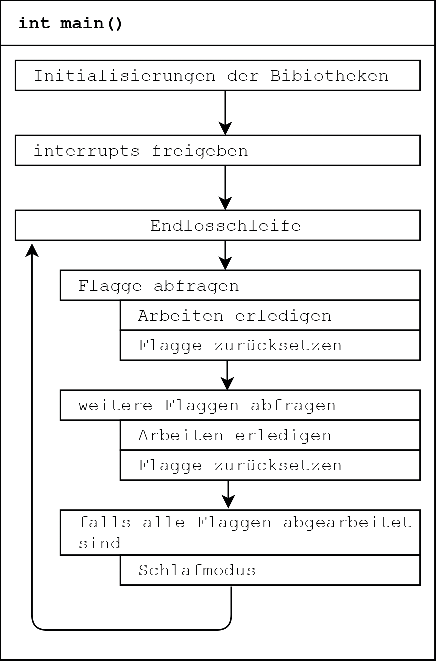
\includegraphics{main_diagram.pdf}
    \caption{Der Grundablauf schematisch dargestellt}
    \label{img:grundablauf}
\end{figure}
\newline
Der Grundablauf ist in Abbildung \ref{img:grundablauf} zusehen. Es wird zuerst der Mikrorechner und alle benötigten Systeme initialisiert und dann in den interrupt-gesteuerten Betrieb übergegangen. Der Prozessor wird also in den Schlaf- bzw. Low-Power-Modus versetzt und reagiert ab sofort nur noch auf auftretende interrupts. Die aufgerufene interrupt service routine (ISR) soll möglichst schnell abgearbeitet werden, also wird meist lediglich das interrupt ausgewertet und dann eine entsprechende Flagge gesetzt. Dann wird der Schlafmodus verlassen und die ISR beendet. Durch das Verlassen des Schlafmodus werden nun in der main()-Funktion die nächsten Befehle ausgeführt. Hier werden nun die Flaggen abgefragt und die entsprechenden Arbeiten erledigt. Sobald alle Flaggen abgefragt und abgearbeitet sind, wird der Prozessor wieder in den Schlafmodus versetzt. Diese Abarbeitung in der main()-Funktion hat den großen Vorteil, dass lang andauernde Arbeiten, wie z.B. Ansteuerung des Displays mit Wartezeiten, durch interrupts unterbrochen werden können, ohne das erst auf die lange andauernden Anweisungen gewartet werden muss. Diese Blockierung der schnell abzuarbeitenden ISRs passiert, wenn alle Aufgaben in ISRs passieren und nicht in der main()-Funktion. Zeitkritische Aufgaben z.B. Tastendrücke oder Töne könnten nicht richtig oder zeitnah ausgelesen bzw. ausgegeben werden. Eine Ausnahme dieser Regel betrifft die \source{play\_tone}-Funktion der Tonbibliothek, siehe .%TODO: ref

\subsection{Modulstruktur}
Die Programmierung des Mikrorechners erfolgte in Teilmodulen, die sich den verschiedenen Teilbereichen des Projekts widmen. Diese Teilmodule des Projekts wurden erst für sich entwickelt und sobald ein passabler Grad der Implementierung erreicht wurde in das Gesamtprojekt eingebunden und im Verbund getestet. Das Projekt wurde in folgende Module zerlegt:
\begin{itemize}
    \item Sequenz-Datenstrukturen (\textsl{sequence.h})
	\item Display-Ansteurung (\textsl{lcd.h})
	\item Eingaben, also Taster und Drehgeber (\textsl{input.h})
	\item Tonerzeugung (\textsl{tone.h})
	\item LED-Matrix (\textsl{led\_matrix.h})
\end{itemize}
Die Steuerung des Programms passiert in der \textsl{main.c} über die Funktionen, die auf die Eingaben des Benutzers reagieren. Dort werden alle Bibliotheken und Module eingebunden und zum Projekt vereinigt.

\section{Module}
Hier werden die Module genauer in ihrem Aufbau und ihrer Struktur beschrieben. Die Modulnamen für die tatsächlichen Dateien sind in Klammern angegeben und umfassen die entsprechende *.h und *.c Dateien.

\subsection{\source{main.c}}
Die \source{main.c}-Datei ist der Einstiegspunkt des Programms und enthält die Funktion \source{int main()}. Es werden alle unserer Bibliotheken inkludiert, und diese werden gleich zu Beginn durch ihre Initialisierungsfunktionen initialisiert werden können. Danach werden die interrupts freigegeben und das Programm startet die Hauptschleife und damit den interrupt-basierten Ablauf, wie im Abschnitt Grundstruktur und in der Abbildung \ref{img:grundablauf} erläutert.
\newline


Es werden außer den ISRs noch ähnliche Funktionen definiert, die durch Bibliotheken für bestimmte Ereignisse aufgerufen werden. Dies sind \source{void new\_minute()}, das von der Uhrzeit-Bibliothek aufgerufen wird, sobald eine neue Minute angebrochen ist und die Funktion \source{void alarm\_ring()}, die signalisiert, dass ein Alarm ausgelöst worden ist und nun klingeln soll. Diese Funktionen wurden in die \source{main.c} Datei verlegt, da diese Ereignisse Veränderungen in mehreren Bibliotheken auslösen: \source{void new\_minute()} bedeutet, dass die Alarme überprüft werden müssen und die LED-Matrix aktualisiert werden muss;
\source{void alarm\_ring()} bedeutet, dass das Menü in den Alarm-Modus übergehen muss und die Melodie des entsprechenden Alarms gestartet wird.


\subsection{Display (\emph{lcd})}
Die Display Bibliothek steuert das LC-Display und stellt verschiedene Methoden zur Beschreibung und Steuerung dessen zur Verfügung.
Außerdem wurden besondere Methoden für diese Projekt implementiert, die die Anzeige an vorher festgelegten Stellen mit bestimmten Werten beschreibt: \source{write\_pitch}, \source{write\_tone\_length} und \source{write\_tempo}.
\newline
Alle Funktionen des Display benötigen (relativ) viel Zeit, um mit dem Display-Controller zu kommunizieren und sollten demnach nicht in Interrupt Service Routinen benutzt werden.
\subsubsection{\source{void lcd\_init()}}
Das LC-Display wird gestartet und initialisiert über die Funktion \source{void lcd\_init()}. Es wird dann die Initialisierungssequenz für das Display gesendet und es für die weitere Verwendung konfiguriert. Es wird das Display geleert und sowohl der Cursor als auch Blinken ausgeschaltet.
\subsubsection{\source{void lcd\_clear()}}
Eine Funktion, die alles Angezeigte vom Display löscht und den Cursor zurück in die obere, linke Ecke (0, 0) setzt. Sollte nicht zu häufig verwendet werden, da es sonst zu störendem Flackern der Anzeige kommt.
\subsubsection{Schreibfunktionen}
Als grundlegenden Schreibfunktionen, um das Display zu verwenden, sind
\begin{itemize}
    \item \source{void lcd\_write(unsigned char character)},
    \item \source{void lcd\_write\_string(unsigned char string[])} und
    \item \source{void lcd\_write\_int(unsigned int number, int digits)}
\end{itemize}
für die verschiedenen wichtigen Datentypen implementiert. Es können einzelne Zeichen (\source{unsigned character}) gesendet werden, sowie ganze strings, also Felder von Zeichen, die jedoch mit dem terminierendem Zeichen \source{0x0} oder \source{'\textbackslash0'} abgeschlossen werden müssen. Dies passiert automatisch, wenn ein string mit doppelten Anführungszeichen angegeben wird. Um Zahlen (\source{int}) anzuzeigen muss noch ein zweites Argument übergeben werden, das die Anzahl der Stellen bestimmt. Falls die Zahl weniger Stellen besitzt, wird der Rest mit Nullen aufgefüllt, also wird beispielsweise bei der Zahl 45 und drei Stellen \lcdtext{045} angezeigt.
\newline
All diese Funktionen schreiben immer ab der aktuellen Position des Cursors und der Cursor ist nach dem Schreiben beim nachfolgenden Zeichen des letzten neu auf das Display geschriebenen Zeichens.

\subsubsection{\source{void lcd\_set\_cursor(unsigned char x, unsigned char y)}}
Der Cursor kann mithilfe der Funktion \source{void lcd\_set\_cursor(unsigned char x, unsigned char y)} an eine beliebige Stelle im Display gesetzt werden. \source{x} steht für die Position innerhalb der Zeile (beginnend mit 0, also maximal 15) und \source{y} für eine der beiden Zeilen (0 oder 1).

\subsubsection{\source{void write\_pitch(unsigned int pitch)}}
Diese Funktion wandelt die als Zahl angegebene Tonhöhe (wie in X erläutert) %TODO: ref
in die gewohnte Notation (Vorzeichen, Notenname und Oktavnummer, z.B. \lcdtext{\#G4}) um. Sie wird dann auf dem Display an der festgelegten Stelle (0, 0 - linke obere Ecke) für die Tonhöhe angezeigt.

\subsubsection{\source{void write\_tone\_length(enum Tone\_length tone\_length)}}
Mithilfe dieser Funktion wird auf dem Display ab der festgelegten Stelle 0, 1 ein Balkendiagramm als Darstellung der Tonlänge angezeigt. Übergeben wird die in \source{sequence.h} festgelegte Enumeration dafür und je nach Wert zeigt der Balken keine bis vier Segemente: beispielsweise \lcdtext{[OOO.]} oder \lcdtext{[....]}.

\subsubsection{\source{void write\_tempo(unsigned int tempo)}}
Diese Funktion schreibt das Tempo als Zahl in bpm an die dafür festgelegte Stelle auf dem Display: 9, 0.

\subsection{Eingabe (\emph{input})}
In der Eingabe-Bibliothek werden die Taster, das Potentiometer und der Drehgeber (auch Encoder) ausgelesen und dem Rest des Programms in Form von Flaggen zur Auswertung zur Verfügung gestellt. Es werden die Interrupts an Port 2 empfangen und ausgelesen, die jeweilige Flagge gesetzt und der Low-Power-Modus beendet, damit die Flaggen sofort ausgelesen und darauf reagiert werden kann.

\subsubsection{\source{void input\_init()}}
Die Funktion initialisiert den Port 2 so, dass die Interrupts ausgelöst werden und damit auf die Eingaben reagiert werden kann. Außerdem wird der Analog-Digital-Umsetzer (engl. ADC) passend konfiguriert, um das Potentiometer auszulesen. Dafür wird das Capture/Compare-Register 0 (CCR0) des Timer A verwendet, das den ADC hunderte Male pro Sekunde zum Auslesen des gerade anliegenden Potentiometerwertes anregt. CCR0 wird dementsprechend konfiguriert und das Auslesen wird in \source{\_\_interrupt void CCR0\_ISR()} angeregt.

\subsubsection{Flaggen}
Es gibt für jeden Taster eine Flagge (\source{bool button\_SW4} bis \source{bool button\_SW1} entsprechend der Tasternummer), eine Flagge \source{potentiometer\_new} für einen neuen Wert des Potentiometers und zwei Flaggen \source{bool encoder\_l} und \source{bool encoder\_r} für die beiden Drehrichtungen des Encoders.

\subsubsection{\source{\_\_interrupt void P2\_ISR()}}
Die ISR für Port 2, die aufgerufen wird, sobald ein Taster oder der Encoder betätigt werden. Dort wird überprüft, ob der Encoder und wenn ja, in welche Richtung er gedreht wurde. Da die Taster prellen, dürfen die Tasterdrücke nicht sofort ausgewertet werden, da ansonsten bei jedem Tastendruck fälschlicherweise viele Tastendrücke erkannt werden würden. Deswegen wird über die Wartefunktion \source{void debounce\_delay()} eine passende Wartezeit vor der Auswertung realisiert. Je nachdem, welcher Taster oder welche Encoder-Richtung erkannt wurde, wird die entsprechende Flagge gesetzt und der Prozessor aus dem Schlafmodus aufgeweckt, um in der \source{main()}-Funktion darauf zu reagieren.

\subsubsection{\source{\_\_interrupt void ADC10\_ISR()}}
Diese Interrupt Service Routine wird immer dann aufgerufen, sobald ein neuer Wert vom ADC gemessen wurde. Dies bedeutet aber nicht notwendigerweise eine Änderung des Wertes also eine Benutzereingabe. Es muss also ein Vergleich mit dem vorherigen Wert stattfinden, deswegen gibt es zwei Variablen: \source{pot\_value} und \source{pot\_value\_old}. Der ADC gibt 10bit-Werte aus, für das Projekt wollen wir aber nur zwischen 16 Werten unterscheiden (die Schritte der Sequenz). Dies entspricht einer 4bit-Zahl, also wird der ADC-Wert um 6 Werte nach rechts bit-verschoben und dann erst in \source{pot\_value} gespeichert. Falls dieser Wert nicht mit \source{pot\_value\_old} übereinstimmt wird die Flagge \source{potentiometer\_new} gesetzt und der Schlafmodus verlassen, um darauf zu reagieren.


\end{document}
